\documentclass{article}
\usepackage{graphicx}
\usepackage{color}
\usepackage{amssymb}
\usepackage{amsmath}
\usepackage{multirow}
\usepackage{multicol}
\usepackage{array}
\usepackage{rotating,capt-of}
\usepackage[small]{caption}
\usepackage{booktabs}
%\usepackage{float} % for placing figures where i want
\usepackage{afterpage}
\usepackage{epsfig, a4wide}
\usepackage{titling} % shifting title
%\usepackage[margin=1in]{geometry}

\usepackage{tikz,graphicx}
\usetikzlibrary{shapes.geometric, arrows}
\usetikzlibrary{shapes.misc, positioning}
\usetikzlibrary{backgrounds}

\definecolor{lavander}{cmyk}{0,0.48,0,0}
\definecolor{violet}{cmyk}{0.79,0.88,0,0}
\definecolor{burntorange}{cmyk}{0,0.52,1,0}

\def\lav{lavander!90}
\def\oran{orange!30}
\def\dgre{dgreen!30}
\def\vio{violet!30}

\tikzstyle{neighbors}=[draw,circle,violet,bottom color=\lav,
                  top color= white, font=\scriptsize,text=violet,minimum width=10pt]
\tikzstyle{queries}=[draw,circle,burntorange, left color=\oran,
                       text=violet,minimum width=30pt]

\tikzstyle{io} = [trapezium, trapezium left angle=70, trapezium right angle=110, minimum width=3cm, minimum height=1cm, text centered, draw=black, color=burntorange,left color=\oran,text=black,font=\Large]

\tikzstyle{res} = [trapezium, trapezium left angle=70, trapezium right angle=110, minimum width=3cm, minimum height=1cm, text centered, draw=black, color=violet,bottom color=\lav, top color=white,text=black,font=\Large]

\tikzstyle{process} = [rectangle, minimum width=3cm, minimum height=1cm, text centered, draw=violet, bottom color=\vio, top color=white,font=\Large]

\tikzstyle{propro} = [rectangle, minimum width=3cm, minimum height=1cm, text centered, draw=violet, bottom color=\dgre, top color=white,font=\Large]

\tikzstyle{grey} = [ rectangle, rounded corners=10pt, bottom color=black!10, top color=black!2,font=\Large]

\tikzstyle{aro} = [->, thick,  shorten >=2pt, shorten <=2pt]



\newcommand{\myparagraph}[1]{
  \paragraph*{\normalfont\itshape #1}\hspace{5pt}}

% strange snos
\definecolor{purple}{RGB}{180,90,200}
\definecolor{dgreen}{RGB}{0,160,0}
\definecolor{turquoise}{RGB}{0,180,140}
\renewcommand\dblfloatpagefraction{0.03}
\renewcommand\topfraction{.95}
\renewcommand\bottomfraction{.95}
\renewcommand\textfraction{.05}
\renewcommand\floatpagefraction{.95}
\renewcommand\dbltopfraction{.95}
\renewcommand\dblfloatpagefraction{.95}
\newcommand{\TODO}[1] {\begingroup\color{red}#1\endgroup}
\newcommand{\SC}[1] {\begingroup\color{purple}#1\endgroup}
\newcommand{\ACC}[1]{\emph{\textbf{#1}}}
\newcommand{\s}[1]{\begin{tiny}#1\end{tiny}}
\newcommand{\url}[1]{\texttt{http://\small #1}}
\newcommand{\maxentscan}{\texttt{MaxEntScan}}
\newcommand{\NEW}[1]{\begingroup\color{black}#1\endgroup}

%% programs
\newcommand{\spps}{\texttt{SPPS}}
\newcommand{\tri}{\texttt{TRI\_tool}}
\newcommand{\lr}{\texttt{LR\_PPI}}

%% databases
\newcommand{\ncbi}{\texttt{NCBI}}
\newcommand{\nega}{\texttt{Negatome Database}}
\newcommand{\kups}{\texttt{KUPS}}

%\newcommand{\tool}{\texttt{rfPRO}}
%\newcommand{\tool}{\texttt{jackProt}}
\newcommand{\tool}{\texttt{ProteinPrompt}}
\newcommand{\website}{\url{proteinformatics.org/\tool}}

\newcommand{\Hsa}{\emph{Homo sapiens}}
\newcommand{\hsa}{\emph{H.sapiens}}

%\journal{Nature}

\setlength{\droptitle}{-5em}

%\bibliographystyle{naturemag}
\title{\tool: fast and accurate prediction of protein-protein-interactions}

\author{ Sebastian Canzler$^{1,3}$, Ren\'{e} Staritzbichler$^{2,3}$}
\date{}



\begin{document}


\maketitle

\vspace{-1.cm}









\begin{samepage}

\section*{Summary}
  Proteins are the 'machines' of the cell, taking on manifold roles as receptors, enzymes, transporters or even molecular factories.
  Most biological processes involve the interaction between proteins, both in healthy systems as well as in disease.
  Therefore, most drugs target proteins and often impact protein-protein interactions - whether intended as desired effect or unexpected as side-effects.

  
  Computation of the binding behaviour of proteins can complement and guide experimental studies as well as the development of protein-based therapeutics.
  However, calculating protein binding in atomic detail is highly time consuming and requires  knowledge about the structures.
  While proteins are complex three-dimensional molecules, their structure, function and also binding behaviour is encoded in their amino acid sequence.
  In turn, the interaction between proteins can be understood to some degree from their sequence alone.
  
  We developed \tool, a tool based on machine learning, using the sequences of protein pairs as input to estimate their tendency to bind.
  The quality of its predictions outperforms any current competitor by far.

  
  For the training of a high quality learning algorithm a comprehensive dataset needs to be collected.
  We exploited all available sources.
  Positive data was gathered from the
  Database of Interacting Proteins (DIP)
  \cite{Salwinski:2004},
  Human Protein Reference Database (HPRD)
  \cite{Keshava_Prasad:2009},
  Protein  Data Bank (PDB) \cite{Berman:2000}, and the University of Kansas Proteomics Service (KUPS) \cite{Chen:2011}.
  Negative data was obtained from the Negatome Database \cite{Blohm:2014}  and the KUPS server.
  After collecting such a broad database, thorough curation was imperative to improve data quality.
  We performed several iterations of filtering and cleanup, both automated in terms of computational tools, as well as through manual inspection.
  
  The key to 'stellar' performance of a learning algorithm lays often in the way, the data is presented to it. 
  Sequences can not be fed directly into learning machines, but need to be translated into descriptors that enable the learning algorithm to spot the patterns, whether a pair of sequences will bind or not.
  We identified auto-correlation profiles of hydrophobicity scales to best capture the binding propensity. 
  Learning algorithms themselves are available in many implementations.
  Most prominent in the current rise of learning applications in biology  are artificial neural networks (ANN).
  However, following an agnostic approach, we compared ANNs with support vector machines and several other learning methods.
  As a result, we found that the random forest approach leads to the cleanest separation of binders and non-binders (see Fig. \ref{fig:training}).
  
  
  \tool\  is available online and free for academic users.
  The server allows users to scan their query sequence against several large databases (27k-118k) for potential binders (see Fig. \ref{fig:workflow} and \ref{fig:webform}).
  Scanning a query sequence against the human database requires around one minute.
  By running \tool\ for several independent queries, interaction networks can be identified (see Fig. \ref{fig:connect}).
  (The server will be ready for testing by the time of submission of the full draft.) 
 
  \centerline{\website} 
  \hspace{1px}
  
  Several competing software-tools are available: \spps\ \cite{Liu:2012}, \tri\ \cite{Perovic:2017}, and \lr\ \cite{Pan:2010}.
  We compared \tool\ with them, using a challenging dataset.
  As a quality measure we applied the area under curve (AUC), derived from receiver operating characteristics (see Fig. \ref{fig:comparison}).
  The AUC is 0.5 for complete noise and 1 for a perfect predictor.
  The other tools reached the following AUC values: \spps: 0.77, \tri: 0.73, \lr: 0.6.
  The outlined procedure resulted in an AUC of 0.94 for \tool.


  

\end{samepage}

\pagebreak

\noindent\textbf{Affiliations:}\\
  { 1) Bioinformatics Group, Department of Computer Science,
  University of Leipzig,
  H{\"a}rtelstra{\ss}e 16-18, 04107 Leipzig, Germany.\\
2) ProteinFormatics Group, Institute of Medical Physics and Biophysics, University of Leipzig,
  H{\"a}rtelstra{\ss}e 16-18, 04107 Leipzig, Germany.\\
3)
Immuthera GmbH, L{\"o}{\ss}niger Stra{\ss}e 16, 04275 Leipzig, Germany.}




\begin{figure}
  \centerline{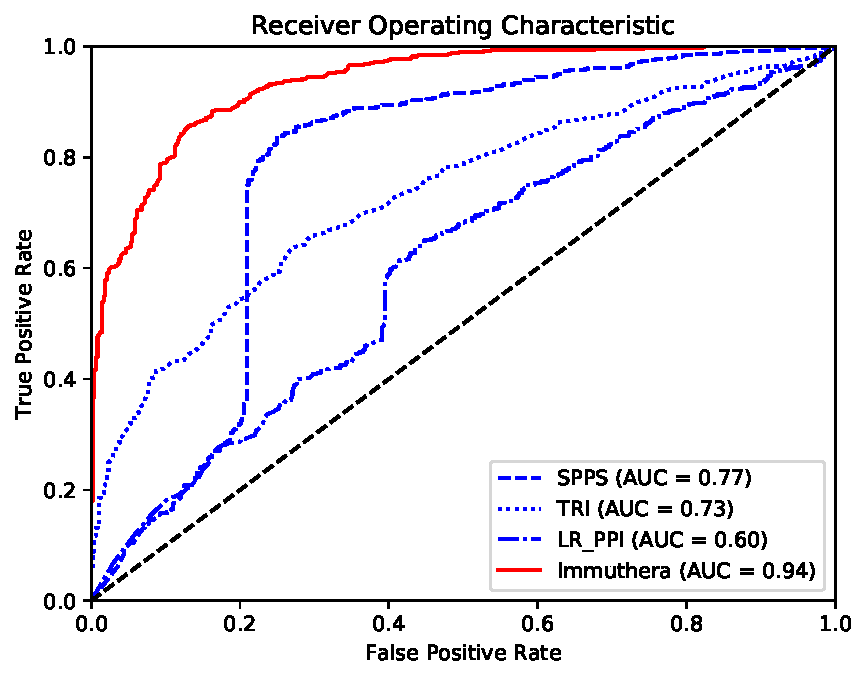
\includegraphics[width=0.7\textwidth]{img/comparison_roc.pdf}}
  \caption{Receiver operating characteristics - an in-depth quality estimation: a perfect predictor would have a rectangular curve, shown in dark green. Complete noise is depicted as light green dashed line. Here, we show a comparison of \tool, \spps, \tri, \lr\ using a test-dataset including 968 protein-protein pairs (excluded from training of method). }
  \label{fig:comparison}
\end{figure}


\begin{figure}
  \iffalse
%\documentclass{article}
%\usepackage{tikz}
%\usetikzlibrary{shapes.geometric, arrows}
%\usetikzlibrary{shapes.misc, positioning}
%
%\definecolor{lavander}{cmyk}{0,0.48,0,0}
%\definecolor{violet}{cmyk}{0.79,0.88,0,0}
%\definecolor{burntorange}{cmyk}{0,0.52,1,0}
%
%\def\lav{lavander!90}
%\def\oran{orange!30}
%
%\tikzstyle{neighbors}=[draw,circle,violet,bottom color=\lav,
%                  top color= white, font=\scriptsize,text=violet,minimum width=10pt]
%\tikzstyle{queries}=[draw,circle,burntorange, left color=\oran,
%                       text=violet,minimum width=30pt]
%
%\tikzstyle{io} = [trapezium, trapezium left angle=70, trapezium right angle=110, minimum width=3cm, minimum height=1cm, text centered, draw=black, color=burntorange,left color=\oran,text=black]
%
%\tikzstyle{res} = [trapezium, trapezium left angle=70, trapezium right angle=110, minimum width=3cm, minimum height=1cm, text centered, draw=black, color=violet,bottom color=\lav, top color=white,text=black]
%
%\tikzstyle{process} = [rectangle, minimum width=3cm, minimum height=1cm, text centered, draw=violet, bottom color=\lav, top color=white]
%
%\tikzstyle{grey} = [ rectangle, rounded corners=10pt, bottom color=black!10, top color=black!2] 
%
%\tikzstyle{aro} = [->, thick,  shorten >=2pt, shorten <=2pt]
%
%\begin{document}
\fi

\hspace{1cm}\begin{tikzpicture}[auto,thick, scale=0.5, transform shape,align=center, node distance = 1.5cm]

  \tikz {every node} = [font=\LARGE]
  
  \node (final) [io] { ProteinPrompt - final predictor};
  \node (apply) [process, below=1cm of final] {Evaluate}
  edge [aro] (final);
  \node (opt) [process,below=1cm of apply] {Optimize};

  \draw [aro,bend right=45] (apply.south) edge (opt.north)
                            (opt.north) edge (apply.south);


  \node[grey,minimum width=11cm,minimum height=11.cm,below left=0.5cm and 0 of opt]{\parbox[b][10.cm]{4cm}{Positive Dataset}};
  
  \node (ptrain) [io,below left=1cm and 3.4cm of opt] {Train}
  edge[aro,bend left=45] (opt.west);

  \node (ptest)  [io,left=1cm of ptrain] {Test}
  edge[aro,bend left=45] (apply.west);

  \path (ptrain) -- node(ppool)[io,below=1.5cm]{Pool} (ptest);

  \draw [aro] (ppool) edge (ptest)
  edge( ptrain);

  \node (pclean) [process,below=1cm of ppool] {Filtering}
  edge[aro](ppool);
  
  
  \node (ip1) [io, below left=1.5cm and 1cm of pclean] {PDB}
  edge[aro](pclean);
  \node (ip2) [io,right=4cm of ip1] {HPRD}
  edge[aro](pclean);
  \node (ip3) [io,below right=0.3cm and 0.1cm of ip1] {DIP}
  edge[aro](pclean);
  \node (ip4) [io,right=0.7cm of ip3] {KUPS}
  edge[aro](pclean);

  \node[grey,minimum width=11cm,minimum height=11.cm,below right=0.5cm and 0 of opt]{\parbox[b][10.cm]{4cm}{Negative Dataset}};

  \node (ntrain) [io,below right=1cm and 3.2cm of opt] {Train}
  edge[aro,bend right=45] (opt.east);

  \node (ntest)  [io,right=1cm of ntrain] {Test}
  edge[aro,bend right=45] (apply.east);

  \path (ntrain) -- node(npool)[io,below=1.5cm]{Pool} (ntest);

  \node (nclean) [process,below=1cm of npool] {Filtering}
  edge[aro] (npool);
  
  \draw [aro] (npool) edge (ntest)
  edge( ntrain);

  \node (ghost) [below=1.5cm of nclean]{};
  \node (in1) [io, below right=1.5cm and 0.2cm of nclean] {Negatome DB}
  edge[aro](nclean);
  \node (in2) [io, below left=1.5cm and 0.7cm of nclean] {KUPS}
  edge[aro](nclean);

  \draw [dotted, shorten <=2pt] (opt) edge (0,-16.1);
  
%  edge[aro, bend right=45] (ptest.north);

\end{tikzpicture}

%\end{document}

  \caption{ Training of the learning algorithm: goal is to distinguish positive data of known binders from negative data of non-binders (depicted by dotted line). Data was collected from PDB, DIP, KUPS, HPRD, and the Negatome DB. Rigorous filtering is crucial for the quality of the data. In order to avoid over-fitting, the datasets have to be split in training and testing data. In an iterative process the performance of the learning algorithm is maximized on the training dataset, while at the same time monitoring the performance on the test-data. Over-fitting starts where the prediction quality for the test-data starts to decrease.}
  \label{fig:training}
\end{figure}


\begin{figure}
  \iffalse
%\documentclass{article}
%\usepackage{tikz,graphicx}
%\usetikzlibrary{shapes.geometric, arrows}
%\usetikzlibrary{shapes.misc, positioning}
%\usetikzlibrary{backgrounds}
%
%
%\definecolor{lavander}{cmyk}{0,0.48,0,0}
%\definecolor{violet}{cmyk}{0.79,0.88,0,0}
%\definecolor{burntorange}{cmyk}{0,0.52,1,0}
%
%\def\lav{lavander!90}
%\def\oran{orange!30}
%
%\tikzstyle{neighbors}=[draw,circle,violet,bottom color=\lav,
%                  top color= white, font=\scriptsize,text=violet,minimum width=10pt]
%\tikzstyle{queries}=[draw,circle,burntorange, left color=\oran,
%                       text=violet,minimum width=30pt]
%
%\tikzstyle{io} = [trapezium, trapezium left angle=70, trapezium right angle=110, minimum width=3cm, minimum height=1cm, text centered, draw=black, color=burntorange,left color=\oran,text=black,font=\Large]
%
%\tikzstyle{res} = [trapezium, trapezium left angle=70, trapezium right angle=110, minimum width=3cm, minimum height=1cm, text centered, draw=black, color=violet,bottom color=\lav, top color=white,text=black,font=\Large]
%
%\tikzstyle{process} = [rectangle, minimum width=3cm, minimum height=1cm, text centered, draw=violet, bottom color=\lav, top color=white,font=\Large]
%
%\tikzstyle{grey} = [ rectangle, rounded corners=10pt, bottom color=black!10, top color=black!2,font=\Large] 
%
%\begin{document}
\fi

\hspace*{1.5cm}
\begin{tikzpicture}[auto,thick, scale=0.6, transform shape,align=left, node distance = 1.5cm]



  \node (result) [res] {Binders};
  \node (prompt) [propro, left=1cm of result] {Random Forrest};
  \node (ac) [propro, left=1cm of prompt] {Autocorrolation};

  \node (seq) [io, left=1.5cm of ac] {Sequence};
  \node (tag) [io, below=0.7 of seq] {Tags};
  \node (db)  [io, below=0.7 of tag] {Database};

  \node (db1) [io, right=2.1cm of db] {Human};
  \node (db2) [io, right=0.5cm of db1] {Mammalia};
  \node (db3) [io, below=0.3cm of db1] {Vertebrata};
  \node (db4) [io, below=0.3cm of db2] {Metazoa};

  
  \begin{scope}[on background layer]
    \node (server) [grey, minimum width = 9.2cm, minimum height=2.4cm, below left=-2cm and -4.1cm of prompt] {\parbox[t][2.1cm]{2.8cm}{\Large  ProteinPrompt}};
    \node (webform) [grey, minimum width = 5cm, minimum height=6cm, below left=-5.6cm and -3cm of db] {\parbox[t][5.7cm]{1.7cm}{\Large  Webform}};
    \node (backdb) [grey, minimum width=10.4cm, minimum height=3.7cm, below left=-2.cm and -3.3cm of db2] {\parbox[t][3.3cm]{5.5cm}{\Large Databases to scan against}};
  \end{scope}

  
  \draw [->, shorten >=2pt, shorten <=2pt] (seq) -- (ac);
  \draw [->, shorten <=2pt, shorten >=22pt] (db) -- (db1);
  \draw [->, shorten >=2pt, shorten <=2pt] (ac) -- (prompt);
  \draw [->, shorten >=2pt, shorten <=2pt] (prompt) -- (result);
  \draw [->, ] (-4.8,-2.1) edge (-4.8,-0.7);


%  \path (seq) |- node(logo)[inner sep=0,above=1.5cm]
%        {
\includegraphics[width=0.4\textwidth]{img/logo_small.jpg}}
%  (n0);

\end{tikzpicture}

%%\end{document}

  \caption{ Work-flow of the \tool\  server: the user has to provide the query sequence, a tag for later identification, and to select the database in which potential binders are expected. \tool\  converts the sequence first into auto-correlation descriptors prior to calling the random forest algorithm.
    The server returns a list of potential binders, sorted by expected binding strength.
     The website displays the results as a table, that can be filtered by keywords and sorted by several criteria. 
    Additionally, a download link is provided. }
  \label{fig:workflow}
\end{figure}

\begin{figure}
  \documentclass{article}
\usepackage{tikz}
\usetikzlibrary{shapes.geometric, arrows}
\usetikzlibrary{shapes.misc, positioning}

\definecolor{lavander}{cmyk}{0,0.48,0,0}
\definecolor{violet}{cmyk}{0.79,0.88,0,0}
\definecolor{burntorange}{cmyk}{0,0.52,1,0}

\def\lav{lavander!90}
\def\oran{orange!30}

\tikzstyle{neighbors}=[draw,circle,violet,bottom color=\lav,
                  top color= white, font=\scriptsize,text=violet,minimum width=10pt]
\tikzstyle{queries}=[draw,circle,burntorange, left color=\oran,
                       text=violet,minimum width=30pt]

\tikzstyle{io} = [trapezium, trapezium left angle=70, trapezium right angle=110, minimum width=3cm, minimum height=1cm, text centered, draw=black, color=burntorange,left color=\oran]

\tikzstyle{process} = [rectangle, minimum width=3cm, minimum height=1cm, text centered, draw=black, bottom color=\lav, top color=white]

\tikzstyle{grey} = [ rectangle, rounded corners=10pt, bottom color=black!10, top color=black!2] 

\begin{document}
\begin{tikzpicture}[auto,thick, scale=0.5, transform shape,align=center, node distance = 1.5cm]

    \node[queries] (n0) at (-4,0) {query};
    \foreach \k/\l/\j in {1/1/2,-1/1/8,1.4/0/3,-1.4/0/7,1/-1/4,-1/-1/6,0/1.4/1,0/-1.4/5}{
        \node[neighbors] (n\j) at (\k-4,\l) {b:\j};
        %      \path (n\i\j) edge (\i);
        \draw (n\j) -- (n0);
    }
  \foreach \x/\y/\i in {1/0/4,7/0/2,4/3/1,4/-3/3} {
    \node[queries] (\i) at (\x,\y) {q:\i};
    \foreach \k/\l/\j in {1/1/2,-1/1/8,1.4/0/3,-1.4/0/7,1/-1/4,-1/-1/6,0/1.4/1,0/-1.4/5}{
        \node[neighbors] (\i\j) at (\x+\k,\y+\l) {b:\i\j};
        %      \path (n\i\j) edge (\i);
        \draw (\i\j) -- (\i);
    }
  }

  \foreach \i in {5,6}{
    \foreach \j in {1,2,3}{
      \draw (2\i) -- (3\j);
      \draw (1\i) -- (4\j);
    }
  }
  
  \foreach \i in {3,4,5}{
    \foreach \j in {1,8}{
      \draw (4\i) -- (3\j);
      \draw (1\i) -- (2\j);
    }
  }
  
  \draw (43) -- (27);


  

  \node (r1) [io, below of=35] {Query 1};
  \node (r2) [io, below of=r1] {Query 2};
  \node (r3) [io, below of=r2] {Query 3};
  \node (r4) [io, below of=r3] {Query 4};

  \node (webform) [grey, minimum width = 4.5cm, minimum height=6.8cm] at (-16.5cm,-7.2 ) {\parbox[t][5.8cm]{1.7cm}{\Large  Webform}};

  \node (server) [grey, minimum width = 7.5cm, minimum height=3cm] at (-10.2cm,-5.5 ) {\parbox[t][2.5cm]{2.5cm}{\Large  ProteinPrompt}};

  \node (result) [io] at (n5 |- r1) {Binders};

  \node (prompt) [process, left=1cm of result] {Random Forrest};

  \node (ac) [process, left=1cm of prompt] {Autocorrolation};

  \node (seq) [io, left=1cm of ac] {Sequence};
  \node (tag) [io, below=0.7 of seq] {Tags};
  \node (db)  [io, below=0.7 of tag] {Database};


  \node (backdb) [grey, right=0.5cm of db, minimum width=12cm, minimum height=2.2cm] {};
  
  \node (db1) [io, right=1cm of db] {Human};
  \node (db2) [io, right=0.5cm of db1] {Non red.};
  \node (db3) [io, right=0.5cm of db2] {Others};
  
\end{tikzpicture}
\end{document}

  \caption{Network tracing: having accumulated the lists for several queries, connectivities and thus complex binding networks can be explored.
   The left graph connects an individual query (orange, center) with its potential binders (magenta).
   The right graph is a schematic description of potential interconnections between multiple independent queries.
   This allows identifying queries that either share binding partners or, on the contrary, bind exclusively to certain partners. }
  \label{fig:connect}
\end{figure}

\begin{figure}
  \hspace{-1.5cm}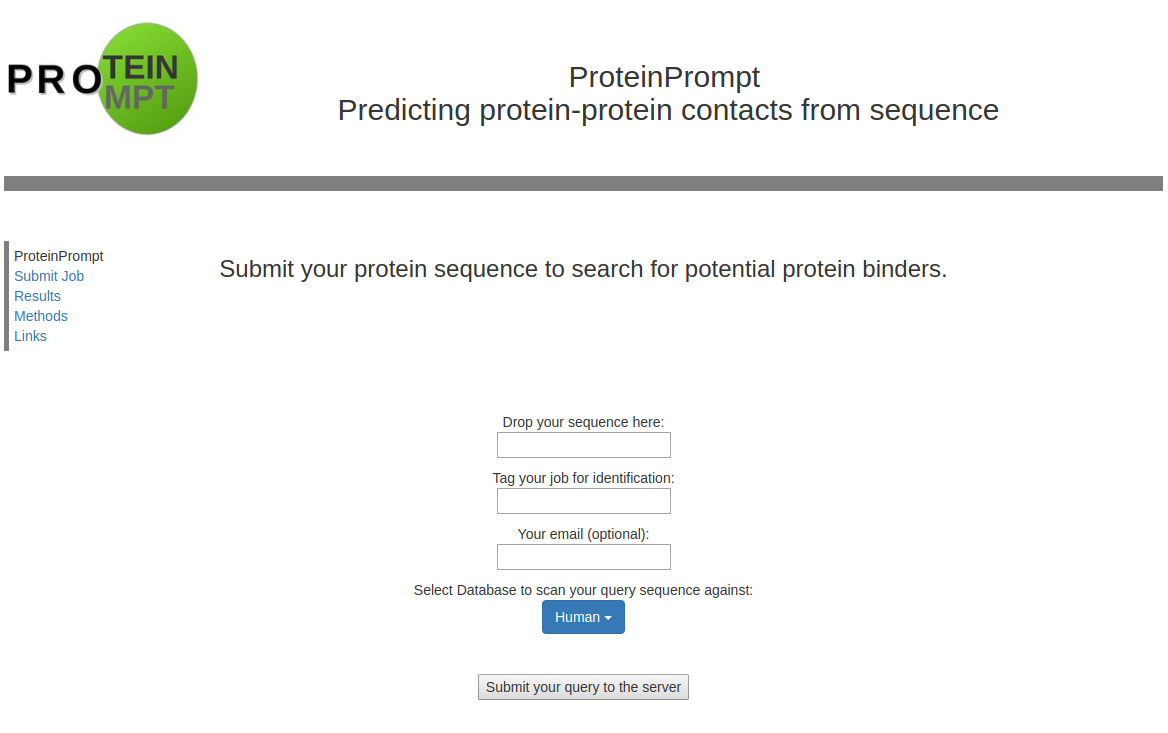
\includegraphics[width=1.2\linewidth]{material/webform.png}
  \caption{ The web-form of \tool.
    Required inputs are the sequence and a tag, allowing to locate results.
    Results will be accessible for 2 weeks.
    By default, the query sequence is scanned against the (filtered) human database, containing $>$27k entries.
    Other organisms can be selected in the drop-down.}
  \label{fig:webform}
\end{figure}


\clearpage
%\onehalfspacing
\bibliographystyle{naturemag}
\bibliography{ppi_prediction}



\end{document}


